\documentclass[12pt]{article}

\setlength\parindent{30pt}
\usepackage[usenames, dvipsnames]{color}
\usepackage{fullpage}
\usepackage{setspace}
\usepackage{amssymb}
\usepackage{amsmath}
\usepackage{caption}
\usepackage{subcaption}
\usepackage{graphicx}
\usepackage[section]{placeins}
\usepackage[utf8]{inputenc}
\usepackage[T1]{fontenc}

\doublespacing


\newcommand{\TODO}[1]{\textcolor{red}{#1}}
\newcommand{\F}[1]{\textcolor{magenta}{#1}}

\newcommand{\contradiction}{{\hbox{%
      \setbox0=\hbox{$\mkern-3mu\times\mkern-3mu$}%
      \setbox1=\hbox to0pt{\hss$\times$\hss}%
      \copy0\raisebox{0.5\wd0}{\copy1}\raisebox{-0.5\wd0}{\box1}\box0
    }}}


\newcommand\Nbb{\mathbb{N}}
\newcommand\Pbb{\mathbb{P}}
\newcommand\Zbb{\mathbb{Z}}
\newcommand\Rbb{\mathbb{R}}
\newcommand\Mcl{\mathcal{M}}

\begin{document}
\title{CMSC 23400}
\author{Patrick Collins, Zachary Jenkins \& Mark Landgrebe}
\date{\today}
\maketitle
\pagebreak

\section{Implementation}

\begin{quote}
  Implementation details: libraries used, server-side component, phone
  or tablet app details, wearable device details, data sources, etc.
\end{quote}

Our implementation is split between a server and a client android
app.

On the server side, we used Python's Flask web framework to manage the
application logic, with persistence provided by MongoDB. We found
MongoDB to be a helpful choice because it provided native support for
location-based queries, in addition to strong integrity checks of
input data. We hosted our server on an AWS instance running Ubuntu
14.04 ``Trusty Tahr.''

On the mobile side, we used Retrofit to develop two RESTful API
clients: first, to access data on our own server, and second, to
consume data from Spotify.

\pagebreak
\section{Challenges}

\begin{quote}
  Challenges, overcome and insurmountable: what did you learn? what
  approaches did you have to adopt? what proved too complex to
  implement or achieve?
\end{quote}

The biggest challenge we faced was Scala, which we attempted to use
for our mobile development. This was a mistake. We discovered that the
Android toolchain was not mature enough for our needs. We had
tremendous trouble trying to build our project, as we found that even
trivial projects hit the 45K dex limit. Eventually we were left to
accept that this was insurmountable and we switched to Java. After
that our development sped up significantly. However we did learn from
this that often maturity is as important or more important than fit
when it comes to choosing tools on a deadline. When using Scala it
felt like we were the first ones to attempt some of what we were
doing, unfortunately that also meant that if it was going to work we
would have to be the first ones to solve the associated problems. In
this way one of the biggest problems was library integration in Scala,
even though Scala is bytecode-compatible with Java.

The next biggest challenge was probably interfacing with multiple
remote forms of communication while also having that influence the
view on screen. We had 3 main remote communications: the server
(including location, songroom information), the Spotify API (for
getting songs, playlists, and user information), and the Spotify
player (for actually playing music) This was mainly a problem because
the view thread cannot be blocked to wait for a request to return
without causing problems with android. This can be solved by having a
thread asnchronously deal with the request. However this solution is
has 2 problems: first, Java threads do not have access to objects
within the scope of their parent, second, Android only the main thread
can change the view. We solved this by building each activity using
the observer pattern, with an observable thread. So the thread would
make asynchronous request to what it needed and when it had the
information it would notify observers, specifically the activity. Then
the activity would launch a runnable on the UIThread which used its
objects to make the necessary changes.

The most insurmountable part of the project was the scope. We started
out with a lot of ideas such as, using sensing with the echo nest to
develop a live music taste profile (an idea we only partially even got
to get into), we also wanted to have a substantial social portion of
the app, including things like matching activity profiles together and
having handshake exchanges of spotify profiles. We also wanted to have
a watch app that integrated all of this in a way that made as much of
it natural and passive as was possible. If we had stayed on our
planned schedule some of this may have been possible. However, we
underestimated how long the core functionality would take to get up
and how long working with new, unknown technologies take to
integrate. The lesson was simply to start with as simple an idea as
possible, execute, and then look at how you can build on top it.

\pagebreak


\section{Future Directions}

\begin{quote}
   If you could do this project again from scratch, what would you do
  differently?
\end{quote}

The obvious is that we would have started with Java as our development
language. However there are several things that we think would have
made our Android development easier, even with a better toolchain. The
first, is that we should have made some abstract Activity classes and
multipurpose views. In a project with a lot of views this is key, we
didn't realize it initially but most of what we doing in every view
branched from a set of ideas, such at the observer pattern mentioned
earlier.

\pagebreak

\section{Lessons Learned}
\begin{quote}
  What have you learned about the themes of the course through working
  on your project?
\end{quote}

One of the biggest things was just the plethora of resources for
finding location. While it seems obvious, this project sought to
crowdsource music DJing, very much in line with the location sensing
themes of this course. What we found in building was very well
documented and a wide variety of location frameworks for both our
mongo backend and our client side android app. This is almost
certainly a capability that has the potenial to see increased use with
increased ability to get location and better battery life to support
constant fixes without fear of destroying battery life.

\pagebreak

\section{Screenshots \& Code }

Our code is available from two separate repositories:
\begin{itemize}
\item Server-side:
  https://github.com/mlandgrebe/CMSC-23400-Project/tree/master
\item Client-side: https://github.com/mlandgrebe/PlaylistrAndroid/tree/Submission
\end{itemize}

\begin{figure}[h]
  \centering
    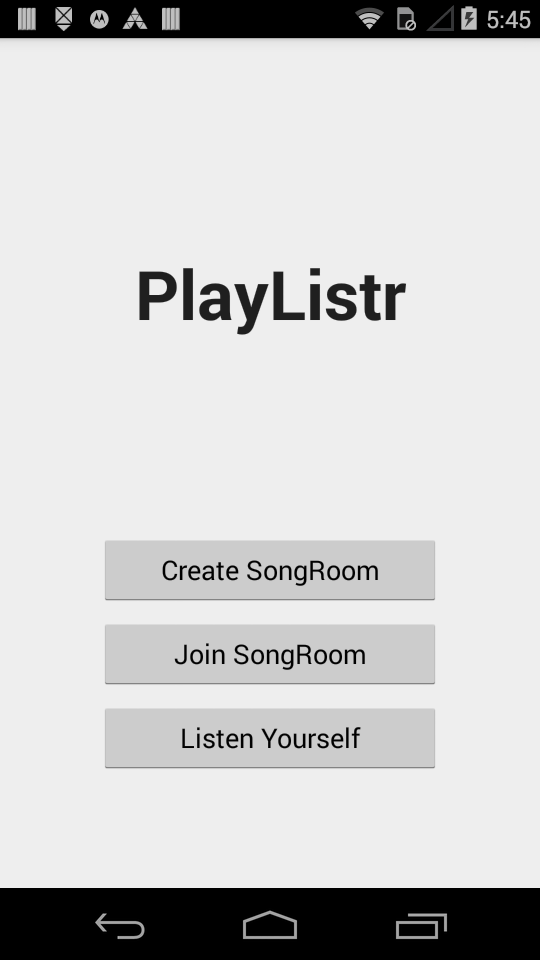
\includegraphics[width=0.5\textwidth]{frontpage}
    \caption{Home Screen}
\end{figure}


\begin{figure}[h]
  \centering
    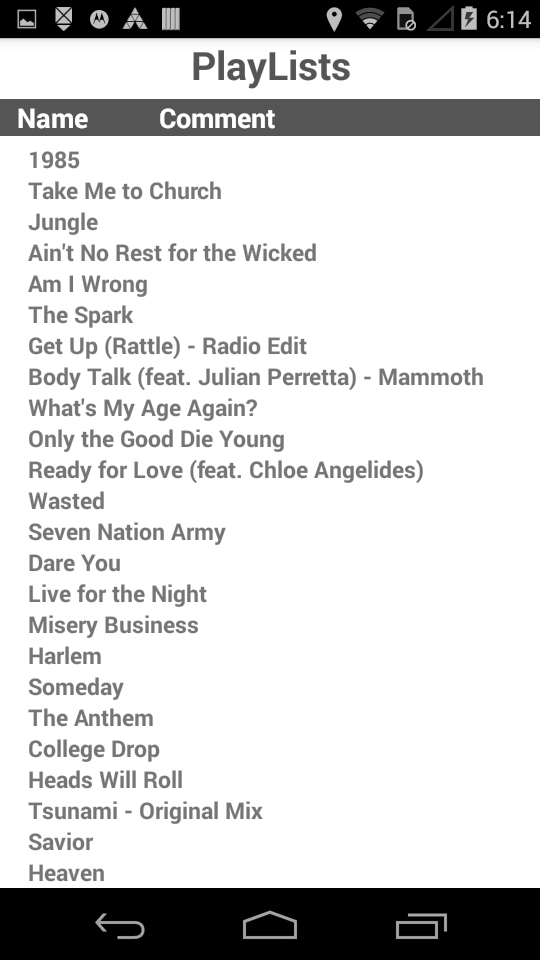
\includegraphics[width=0.5\textwidth]{playlists}
    \caption{Playlist Explorer}
\end{figure}

\begin{figure}[h]
  \centering
    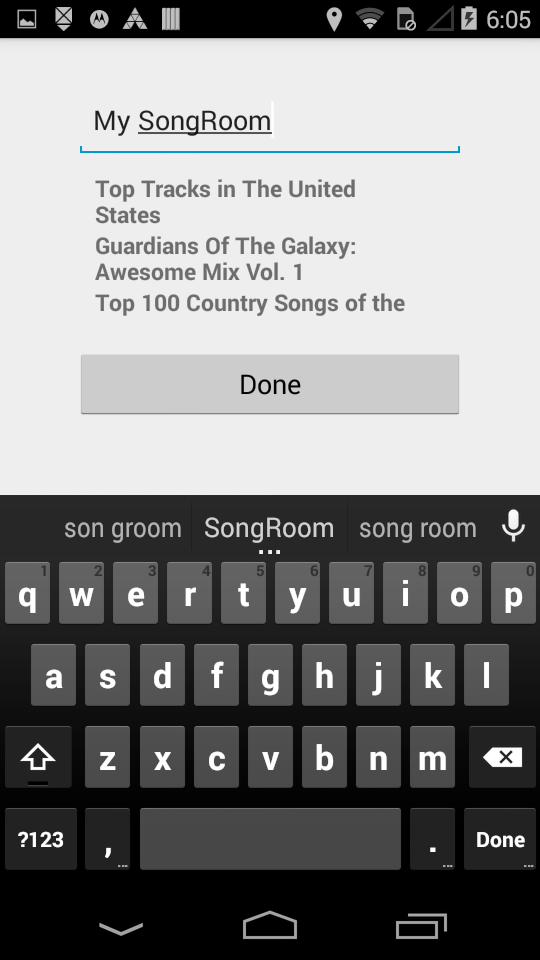
\includegraphics[width=0.5\textwidth]{create-sr}
    \caption{Song Room Creation Menu}
\end{figure}

\begin{figure}[h]
  \centering
    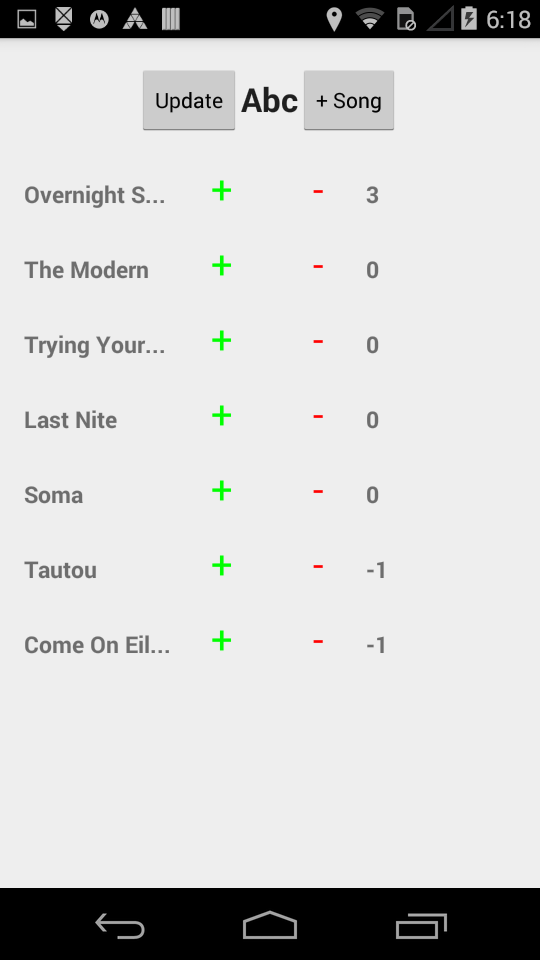
\includegraphics[width=0.5\textwidth]{in-sr}
    \caption{Song Room Lobby}
\end{figure}


\end{document}
